\chapter{Implementation}\label{chapter:Implementation}

In this chapter we describe several approaches to improve the Genetic Solver by parameter tuning.
We will concentrate on solving the problem with \textbf{5 minutes} timeout and the following properties:
\begin{itemize}
	\item \textbf{Software variants: 10;}
	\item \textbf{Number of requests: 15;}
	\item \textbf{Component tree depth: 2;}
	\item \textbf{Resources ratio: 5;}
\end{itemize}
on an Intel Core i7-8700 CPU machine with 64Gb of memory using Fedora Server 29 and OpenJDK 1.8.0 201-b09 for \textbf{5 repetitions} for statistical significance.

Our goal is to achieve valid results in terms of contract violations, and then get an optimal or near-optimal solution in terms of energy consumption. 

We mark base~\footnote{As a base version, we took version at the master branch from 24.09.2019, commit: \href{https://git-st.inf.tu-dresden.de/mquat/mquat2/commit/57845c126c30a1ea59cb35eb16af0bd37930dda9}{57845c126c30a1ea59cb35eb16af0bd37930dda9}} version of the genetic solver as \textbf{B} (Base).


\begin{figure}
	\centering
	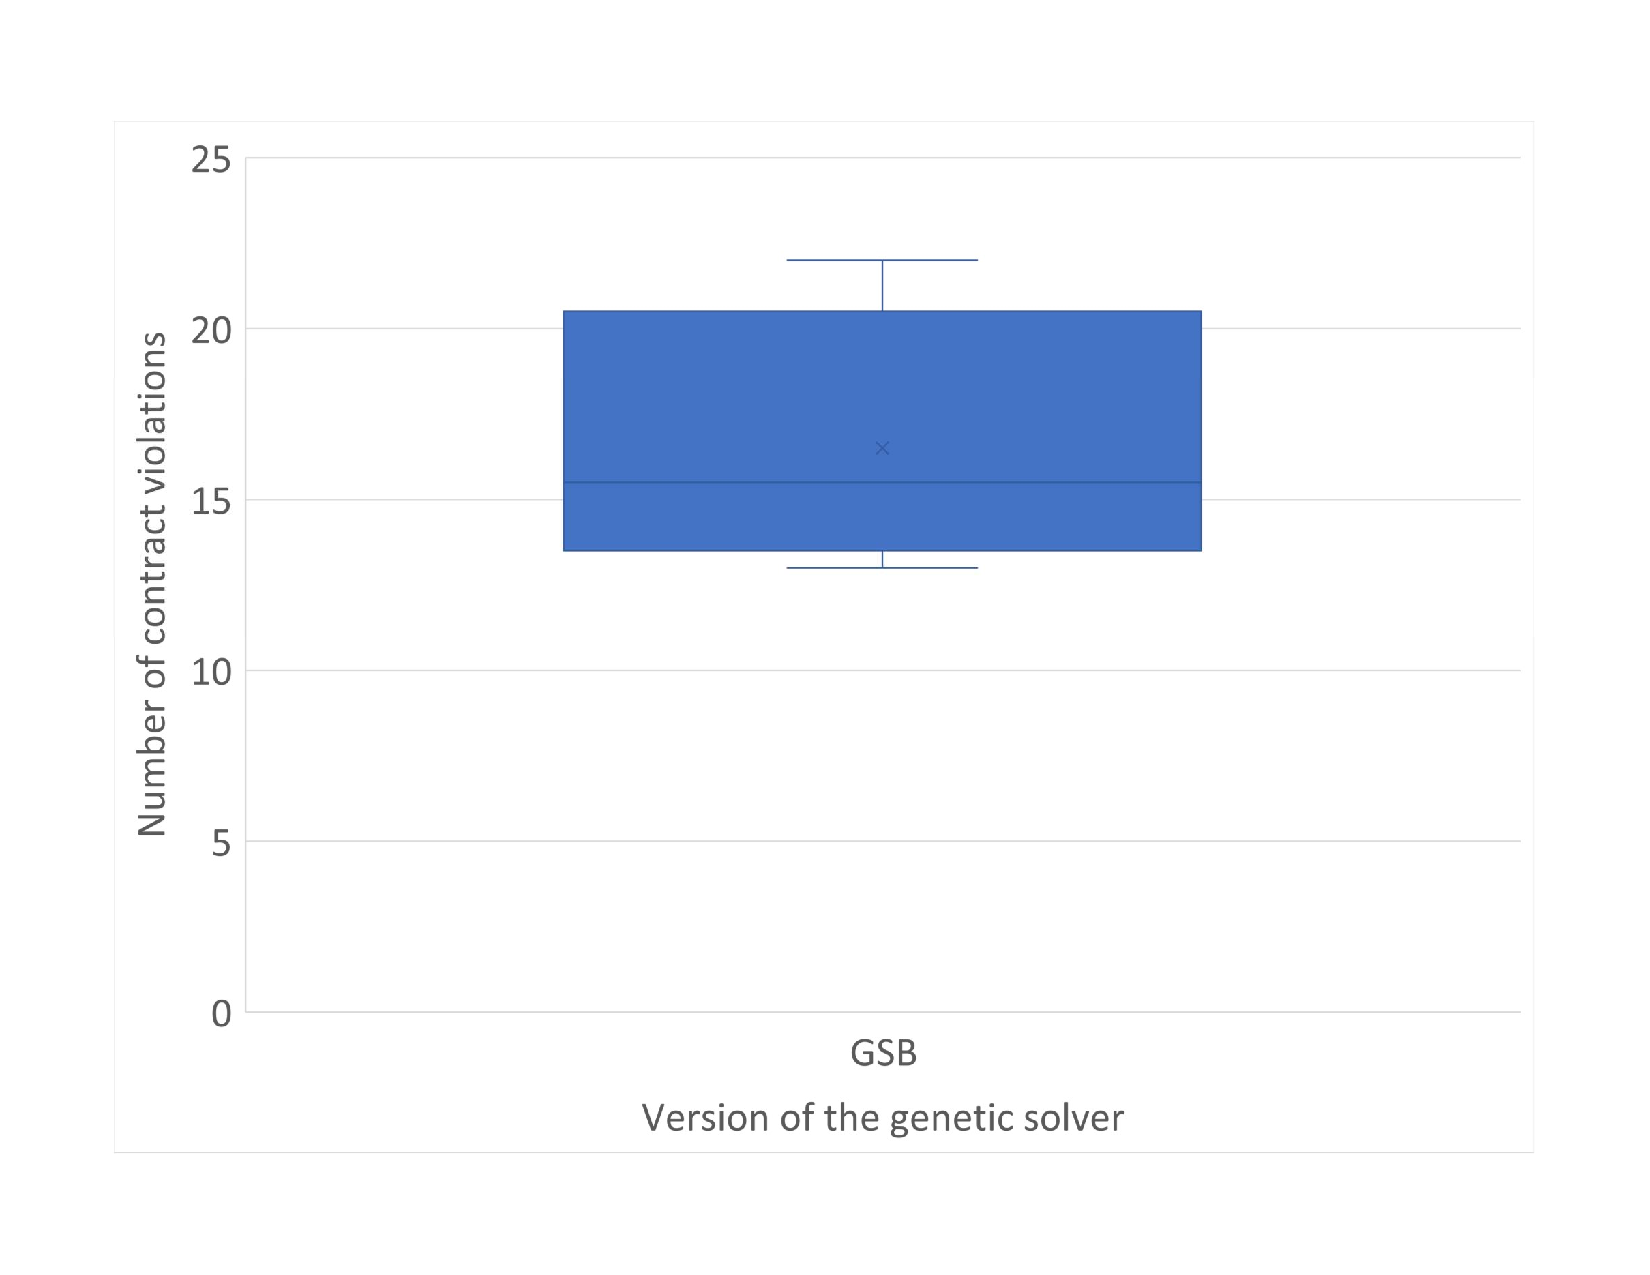
\includegraphics[width=\textwidth]{images/BoxPlotSolverBasic}
	\caption[Box-plot of contract violations for the base version of genetic solver]{Box-plot of contract violations for the base version of genetic solver}
	\label{fig:boxplotsolverbasic}
\end{figure}


Figure~\ref{fig:boxplotsolverbasic} shown the box-plot of the number of contract violations in the base~(\textbf{B}) version of the Genetic Solver. This plot shows that  the base~(\textbf{B}) version solves this task with the number of contract violations in a range from 13 to 22. As a result, there are no valid solutions for the current problem.




\section{First parameter tuning}

The first step to improve the genetic solver was a parameter tuning. To get a set of optimized parameter values it is needed to perform a few essential steps:

\begin{enumerate}
	\item Analyze the genetic solver to find all parameters that could be changed externally. They will be hyperparameters that BRISE will tune.
	\item Adapt BRISE to work with the genetic solver.
	\item Prepare Experiment description for BRISE.
	\item Run BRISE to get the near-optimal configuration of the Genetic Solver.
\end{enumerate}

\textbf{Step 1} involves the analysis of the solver for the presence of parameters that can be changed externally. After diving into the code of the genetic solver, the list of parameters was prepared. Each parameter has a name, short name that consist of capital \textbf{R} and the order number of parameters, the default value that was used in the genetic solver and a range of values for continues parameters or list of values for categorical parameters. The possible value we show with square brackets near the short name. There are:
\paragraph{\texttt{SelectorType}~(R1)~[NSGA2, SPEA2]} — type of the selector algorithm, mentioned in section~\ref{sec:GeneticAlgorithm:Selector}. Default value is \textit{NSGAII};
\paragraph{\texttt{Generations}~(R2)~[Integer]} — number of generations, performed by the genetic solver, working as a termination condition. In this thesis we use only timeout termination. Let us set this parameter in a way, that it does not influence the termination (since the timeout-based termination is used instead);
\paragraph{\texttt{PopulationSize}~(R3)~[100-5000]~[Integer]} — The parameter, that describes the number of individuals in a population. Default value is \textbf{500}. \\

Adaptation of the genetic solver to work in BRISE (\textbf{Step 2}) consists of preparing the executable file of the genetic solver and implementing a method for the worker, which encapsulates execution of the Genetic Solver with specified parameters and returns the results with a number of contract violations and energy consumption.

\textbf{Step 3} means that a user describes hyperparameters that need to be optimized and BRISE components configuration such as selector, repeater, model, and stop condition, list of hyperparameters described by a name, a range of values, or a set of values, the default value.

For parameter tuning of the genetic solver, we use Sobol sampling as a selector algorithm to get the new configuration of hyperparameters, student repeater with a minimal number of measurements — 3 and max number - 6. BRISE uses Bayesian Optimization~(BO) as a prediction model.
To stop BRISE, we use a combination of time-based stop condition with timeout — 12 hours and guaranteed stop condition, which ensures achieving the better result in comparison with the default set of parameters. The experiment description file is presented in Appendix~\ref{appendix:ExperimentDescription}.

We use parameter values of the base~(\textbf{B}) version of the Genetic Solver as a default configuration for BRISE. Such decision makes it possible to use a guarantee stop condition. The default parameter values are presented in Table~\ref{tab:Parameters_B-T}. Also, there are a few parameters in gray-colored filling that have a hard-coded value, but we will discuss them in the next section. 

We mark current version~\footnote{commit: \href{https://git-st.inf.tu-dresden.de/mquat/mquat2/commit/e103f52b3333900d61c6218a1f2ca811bca10289}{e103f52b3333900d61c6218a1f2ca811bca10289}} of the genetic solver as \textbf{B-T}(Base-Tuned).


\begin{table}
	\centering
	\caption{Parameters of B and B-T versions of the Genetic Solver}\label{tab:Parameters_B-T}
	\resizebox{\textwidth}{!}{
		\begin{tabular}{c c c a a a a a a a a a a}
			\hline
			\rotatebox{0}{Genetic Solver} & \rotatebox{0}{\texttt{R1}} & \rotatebox{0}{\texttt{R3}} & \rotatebox{0}{\texttt{R4}} & \rotatebox{0}{\texttt{R5}} & \rotatebox{0}{\texttt{R6}} & \rotatebox{0}{\texttt{R7}} & \rotatebox{0}{\texttt{R8}}  & \rotatebox{0}{\texttt{R9}}  & \rotatebox{0}{\texttt{R10}} & \rotatebox{0}{\texttt{R11}} & \rotatebox{0}{\texttt{R12}} & \rotatebox{0}{\texttt{R13}} \\
			\hline            
			B & NSGA2 & 500 & 0.1 & 0.95 & 0.1 & 0.45 & 0.5 & 0.8 & 0.5 & 0.5 & 50 & 100 \\
			B-T & NSGA2 & 1533 & 0.1 & 0.95 & 0.1 & 0.45 & 0.5 & 0.8 & 0.5 & 0.5 & 50 & 100 \\
			\hline
		\end{tabular}
	}
\end{table}

\begin{figure}
	\centering
	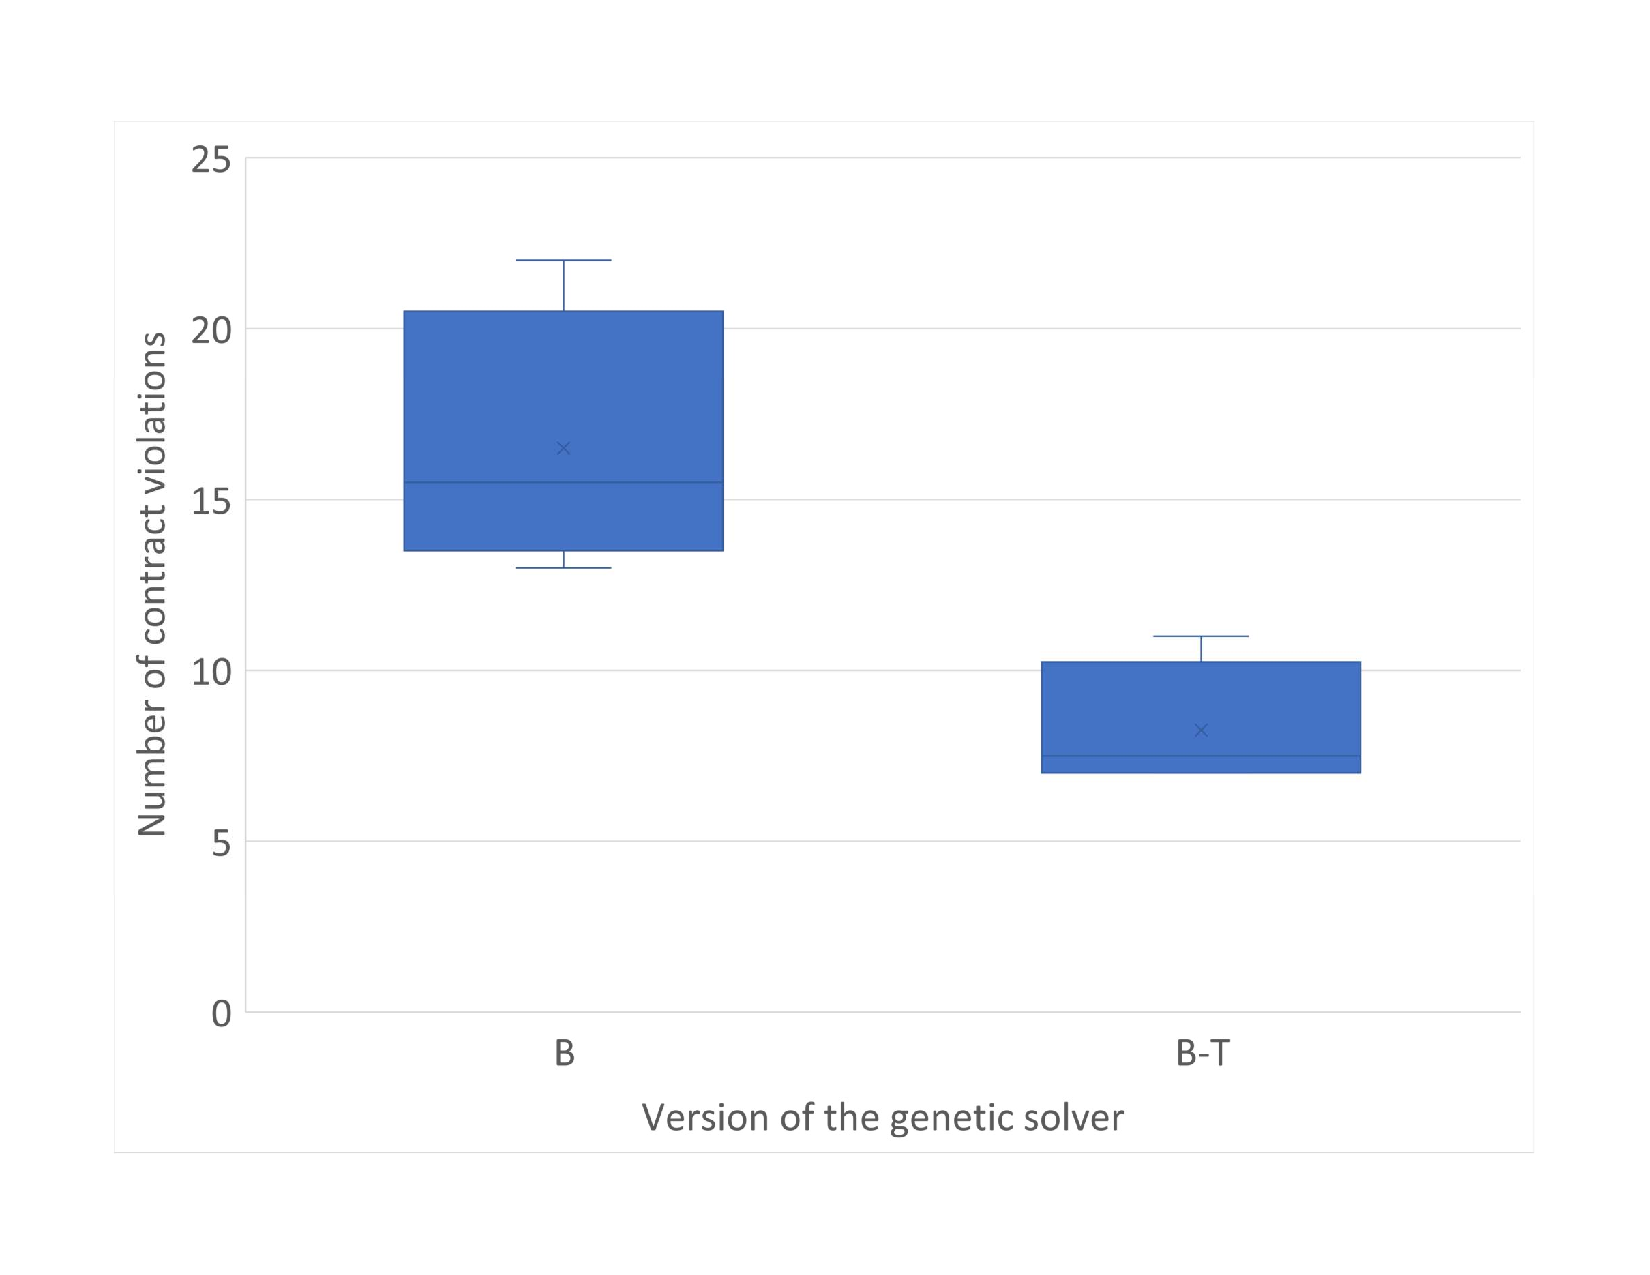
\includegraphics[width=\textwidth]{images/BoxPlotSolverBasicTuning}
	\caption[Box-plot with a number of contract violations for the base version of the Genetic Solver with tuned parameters]{Box-plot with a number of contract violations for the base version of the Genetic Solver with tuned parameters}
	\label{fig:boxplotsolverbasictuning}
\end{figure}

The result of hyperparameter optimization is presented in the Table~\ref{tab:Parameters_B-T}. As showed, BRISE gives a set of parameters with a bigger number of population size~(R3).

The results of solving the earlier described problem as a box-plot showed in Figure~\ref{fig:boxplotsolverbasictuning}. In the Figure~\ref{fig:boxplotsolverbasictuning} also showed a comparison between the base~(\textbf{B}) and its tuned~(\textbf{B-T}) version of the genetic solver. The \textbf{B-T} version of the genetic solver gives a better result compared with the \textbf{B} version. The minimal number of contract violations in the \textbf{B-T} version is almost 2 times fewer than in B version. 

Received results answer the \textbf{RQ1}. Parameter tuning improves results, and it has a positive effect on the genetic solver, but results are still not valid. 

\section{More parameters}

In the previous section, we showed that not all parameters of the genetic solver exposed for tuning. To make them changeable externally, we use \texttt{GoogleGuiceDependencyInjection}\footnote{\url{https://github.com/google/guice}} tool to change the values of these parameters during the solver call. Let us discuss these parameters:
\paragraph{\texttt{lambda}~(R4)~[0.0-1.0]~[Float]} — as mentioned in Section~\ref{sec:GeneticAlgorithm:Selector}, it is the number of new offspring per generation. We use this parameter as a part of the population size. The default value is 0.1.
\paragraph{\texttt{CrossoverRate}~(R5)~[0.0-1.0]} — as mentioned in section~\ref{sec:GeneticAlgorithmCrossover}, it describes the probability of two individuals to gene exchange. The default value is 0.95.
\paragraph{\texttt{mu}~(R6)~[0.0-1.0]~[Float]} — as mentioned in section~\ref{sec:GeneticAlgorithm:Selector}, it describes the number of parents, selected by the selector to create new individuals. We use this parameter as a part of the population size. The default value is 0.1.
\paragraph{\texttt{MutationRate}~(R7)~[0.0-1.0]~[Float]} — as mentioned in section~\ref{sec:GeneticAlgorithmMutation}, it describes the probability of the individual to mutate. BRISE will tune this parameter with default value 0.45 from the base~(\textbf{B}) version of the genetic solver.
\paragraph{\texttt{ResourceMutationProbability}~(R8)~[0.0-1.0]~[Float]} - the likelihood that during the mutation, the assigned resource will mutate. BRISE will tune this parameter with default value 0.5 from the B version of the genetic solver.
\paragraph{\texttt{CrossoverProbability}~(R9)~[0.0-1.0]~[Float]} — it describes the probability of doing crossover that checks in the crossover operator. The default value of this parameter is 0.8. This parameter was removed in later versions of the genetic solver because it duplicates the functionality of \texttt{CrossoverRate}~(R5). This fact answers \textbf{RQ2}. It is one bad design choice that we want to find, according to \textbf{RQ2}.\\ 


Within the genetic solver evaluator, two factors penalize the quality of the solution in the case of a contract breach or errors in dependencies in the software tree. These coefficients were not set for external tuning. The default value for all parameters is 0.5.
\paragraph{\texttt{ValidityWeight}~(R10)~[0.0-1.0]~[Float]} — coefficient that shows how each contract violation decreases the quality of the solution.
\paragraph{\texttt{SoftwareValidityWeight}~(R11)~[0.0-1.0]~[Float]} — coefficient that shows how each error in the software tree decrease the quality of the solution.\\

As described in Section~\ref{sec:GeneticSolver}, a creator creates random individuals for the initial population.
This method has two features that are necessary to obtain better individuals at the initial stage. These features have parameters:
\paragraph{\texttt{RandomSoftwareAssignmentAttempts}~(R12)~[1-1000]~[Integer]} — max number of attempts to set a valid software tree to the individual on the creation phase. The default value is 50.
\paragraph{\texttt{populateSoftwareSolutionAttempts}~(R13)~[1-1000]~[Integer]} —  max number of attempts to assign software components and resources to get a valid individual on the creation phase. The default value is 100.\\

We mark this version~\footnote{commit: \href{https://git-st.inf.tu-dresden.de/mquat/mquat2/commit/e1db4a941622f9a6609ffcfb5d05df9e7abaffc2}{e1db4a941622f9a6609ffcfb5d05df9e7abaffc2}} of the genetic solver as \textbf{WHC-T}(Without Hard-Code-Tuned).

After optimization, we use an optimized set of values of hyperparameters from BRISE, showed in Table~\ref{tab:Parameters_NHC-T}, as parameters for the \textbf{WHC-T} version genetic solver. As shown with more parameters, BRISE suggests using the \textit{SPEA2} selector algorithm, but the value of the \texttt{CrossoverRate}~(R5) is not changed.

\begin{table}
	\centering
	\caption{Parameters of WHC-T version of the genetic solver}\label{tab:Parameters_NHC-T}
	\resizebox{\textwidth}{!}{
		\begin{tabular}{c c c c c c c c c c c c c}
			\hline
			\rotatebox{0}{Genetic solver} & \rotatebox{0}{\texttt{R1}} & \rotatebox{0}{\texttt{R3}} & \rotatebox{0}{\texttt{R4}} & \rotatebox{0}{\texttt{R5}} & \rotatebox{0}{\texttt{R6}} & \rotatebox{0}{\texttt{R7}} & \rotatebox{0}{\texttt{R8}}  & \rotatebox{0}{\texttt{R9}}  & \rotatebox{0}{\texttt{R10}} & \rotatebox{0}{\texttt{R11}} & \rotatebox{0}{\texttt{R12}} & \rotatebox{0}{\texttt{R13}} \\
			\hline            
			WHC-T & SPEA2 & 2014 & 0.98 & 0.95 & 0.58 & 0.02 & 0.64 & 0.3 & 0.95 & 0.17 & 79 & 266 \\
			\hline
		\end{tabular}
	}
\end{table}

Results of the WHC-T version of the genetic solver presented as box-plot in comparison with earlier versions~(\textbf{B}, \textbf{B-T}) is shown in Figure~\ref{fig:boxplotsolverNoHardcodedTuning}. This box-plot shows that the WHC-T version of the genetic solver is better in comparison to B-T. The max number of contract violations in WHC-T is \textbf{7}. This number is equal to a minimum number of contract violations from the B-T version. But solutions are still \textbf{not valid} for the current problem. 

\begin{figure}
	\centering
	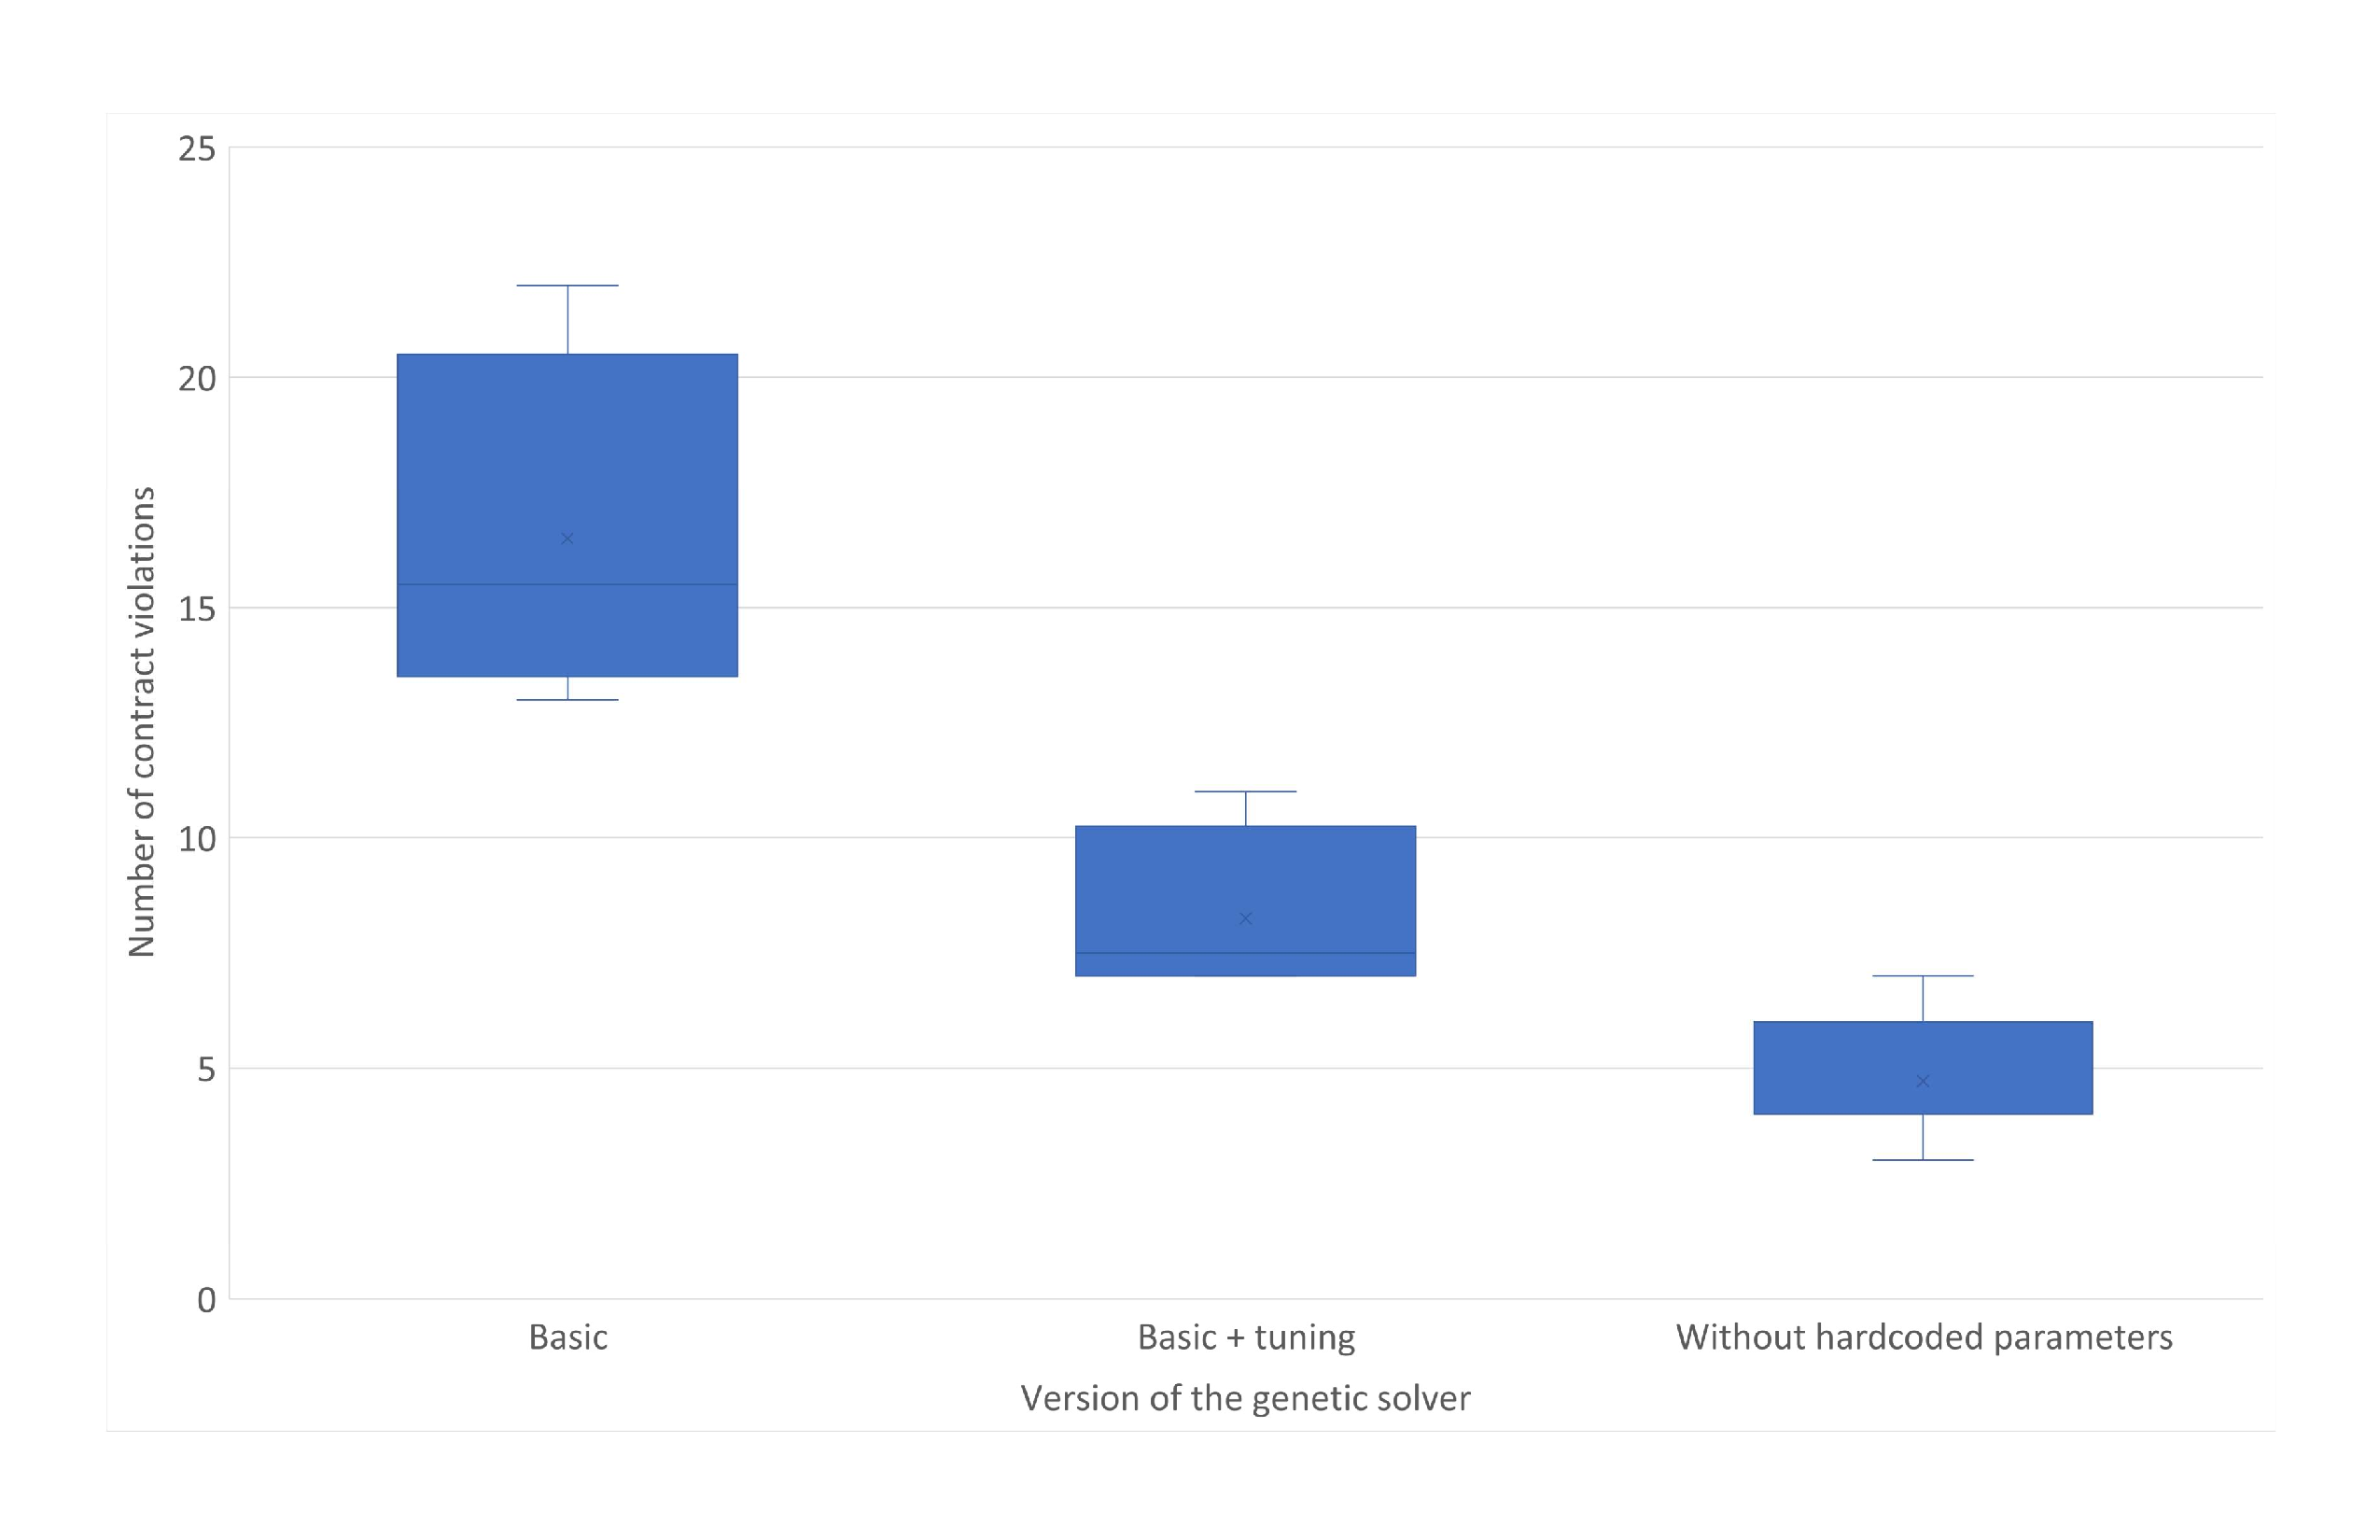
\includegraphics[width=\textwidth]{images/BoxPlotSolverNoHardcodedTuning.pdf}
	\caption[Box-plot with a number of contract violations for the genetic solver without hardcoded parameters in comparison with previous versions]{Box-plot with a number of contract violations for the genetic solver without hard-coded parameters in comparison with previous versions}
	\label{fig:boxplotsolverNoHardcodedTuning}
\end{figure}

This section shows how correctly selected parameter values affect the result of the algorithm in terms of solution validity. For the described problem without complex changes in the algorithm, we got a result which in the worst-case, gave a solution that is almost twice as good as the best solution in the B version of the genetic solver. However, parameter optimization is not enough to obtain valid solutions for the tasks described at the beginning of this chapter. 

\section{New Parameters}\label{sec:NP}

Since the parameter tuning from the previous steps do not give us valid results, we decided to use a parameter engineering approach.
Detailed analysis of crossover and mutation operators showed that the crossover point and the mutation points are coarse-grained. The principle how these points defines described in Section~\ref{sec:GeneticAlgorithmCrossover} and Section~\ref{sec:GeneticAlgorithmMutation}.

We add a few more parameters to crossover and mutation operators. These are probabilities, that allow change of the crossover/mutation points location in different ways in the Tree Shape Genotype.
There are:
\paragraph{\texttt{CrossoverOnRandomChildProbability}~(R14)~[0.0-1.0]~[Float]} — the chance that crossover will occur on the random child or both children otherwise~(since the MQuAT problem constraints described in Section~\ref{sec:MQuATProblem}).
\paragraph{\texttt{CrossoverOnRandomLevelProbability}~(R15)~[0.0-1.0]~[Float]} — the probability that describes a chance to do a crossover on random level of the tree, 
\paragraph{\texttt{CrossoverOnRandomRequestProbability}~(R16)~[0.0-1.0]~[Float]} — the chance to do a crossover on random request,
\paragraph{\texttt{MutationOnRandomChildProbability}~(R17)~[0.0-1.0]~[Float]} — the probability that describes a chance of mutation on a random child,
\paragraph{\texttt{MutationOnRandomLevelProbability}~(R18)~[0.0-1.0]~[Float]} — the chance of mutation on a random level of the tree shape genotype.

The default value for there probabilities, except \texttt{Cross\-ov\-er\-On\-Ran\-dom\-Re\-qu\-est\-Pro\-ba\-bi\-li\-ty}~(R16), is 0.5. For the \texttt{CrossoverOnRandomRequestProbability}~(R16) is 0.0. These values we received empirically during developing.

This version~\footnote{commit: \href{https://git-st.inf.tu-dresden.de/mquat/mquat2/commit/817f7f1ef06f3acbbb4d5e24e32a26c5e6abc4b5}{817f7f1ef06f3acbbb4d5e24e32a26c5e6abc4b5}} of the genetic solver marked as \textbf{NP}(New Probabilities).

The set of parameters used during development is presented in Table~\ref{tab:Parameters_NP-T}. New parameters have the values described above. Furthermore, previously discussed parameters have values from the B version of the genetic solver. That means that all parameters are not tuned.

\begin{table}
	\centering
	\caption{Parameters of NP and NP-T versions of the genetic solver}\label{tab:Parameters_NP-T}
	\resizebox{\textwidth}{!}{
		\begin{tabular}{c c c c c c c c c c c c c c c c c}
			\hline
			\rotatebox{0}{Genetic solver} & \rotatebox{0}{\texttt{R1}} & \rotatebox{0}{\texttt{R3}} & \rotatebox{0}{\texttt{R4}} & \rotatebox{0}{\texttt{R5}} & \rotatebox{0}{\texttt{R6}} & \rotatebox{0}{\texttt{R7}} & \rotatebox{0}{\texttt{R8}}  & \rotatebox{0}{\texttt{R10}} & \rotatebox{0}{\texttt{R11}} & \rotatebox{0}{\texttt{R12}} & \rotatebox{0}{\texttt{R13}} &
			\rotatebox{0}{\texttt{R14}} &
			\rotatebox{0}{\texttt{R15}} &
			\rotatebox{0}{\texttt{R16}} &
			\rotatebox{0}{\texttt{R17}} &
			\rotatebox{0}{\texttt{R18}} \\
			\hline            
			NP & NSGA2 & 500 & 0.1 & 0.95 & 0.1 & 0.45 & 0.5 & 0.5 & 0.5 & 50 & 100 & 0.5 & 0.5 & 0.0 & 0.5 & 0.5 \\
			NP-T & NSGA2 & 2550 & 0.5 & 0.5 & 0.5 & 0.5 & 0.5 & 0.5 & 0.5 & 500 & 500 & 0.5 & 0.5 & 0.5 & 0.5 & 0.5 \\
			\hline
		\end{tabular}
	}
\end{table}

The result of the \textbf{NP} version of the genetic solver presented as box-plot in comparison with earlier versions~(\textbf{B}, \textbf{B-T}, \textbf{WHC-T}) shown in Figure~\ref{fig:boxplotsolverNewParameters}. If we compare the \textbf{B} and the \textbf{NP} versions, then both versions have non-optimized parameter values. The NP version has a minimal number of contract violations equal 3. It is \textbf{3} times less violations than in the best case if the \textbf{B} version. Moreover, this version of the genetic solver has results comparable to the results after parameter tuning in the \textbf{WHC-T} version. We can conclude, that better-designed parameters could also improve the target system. 

\begin{figure}
	\centering
	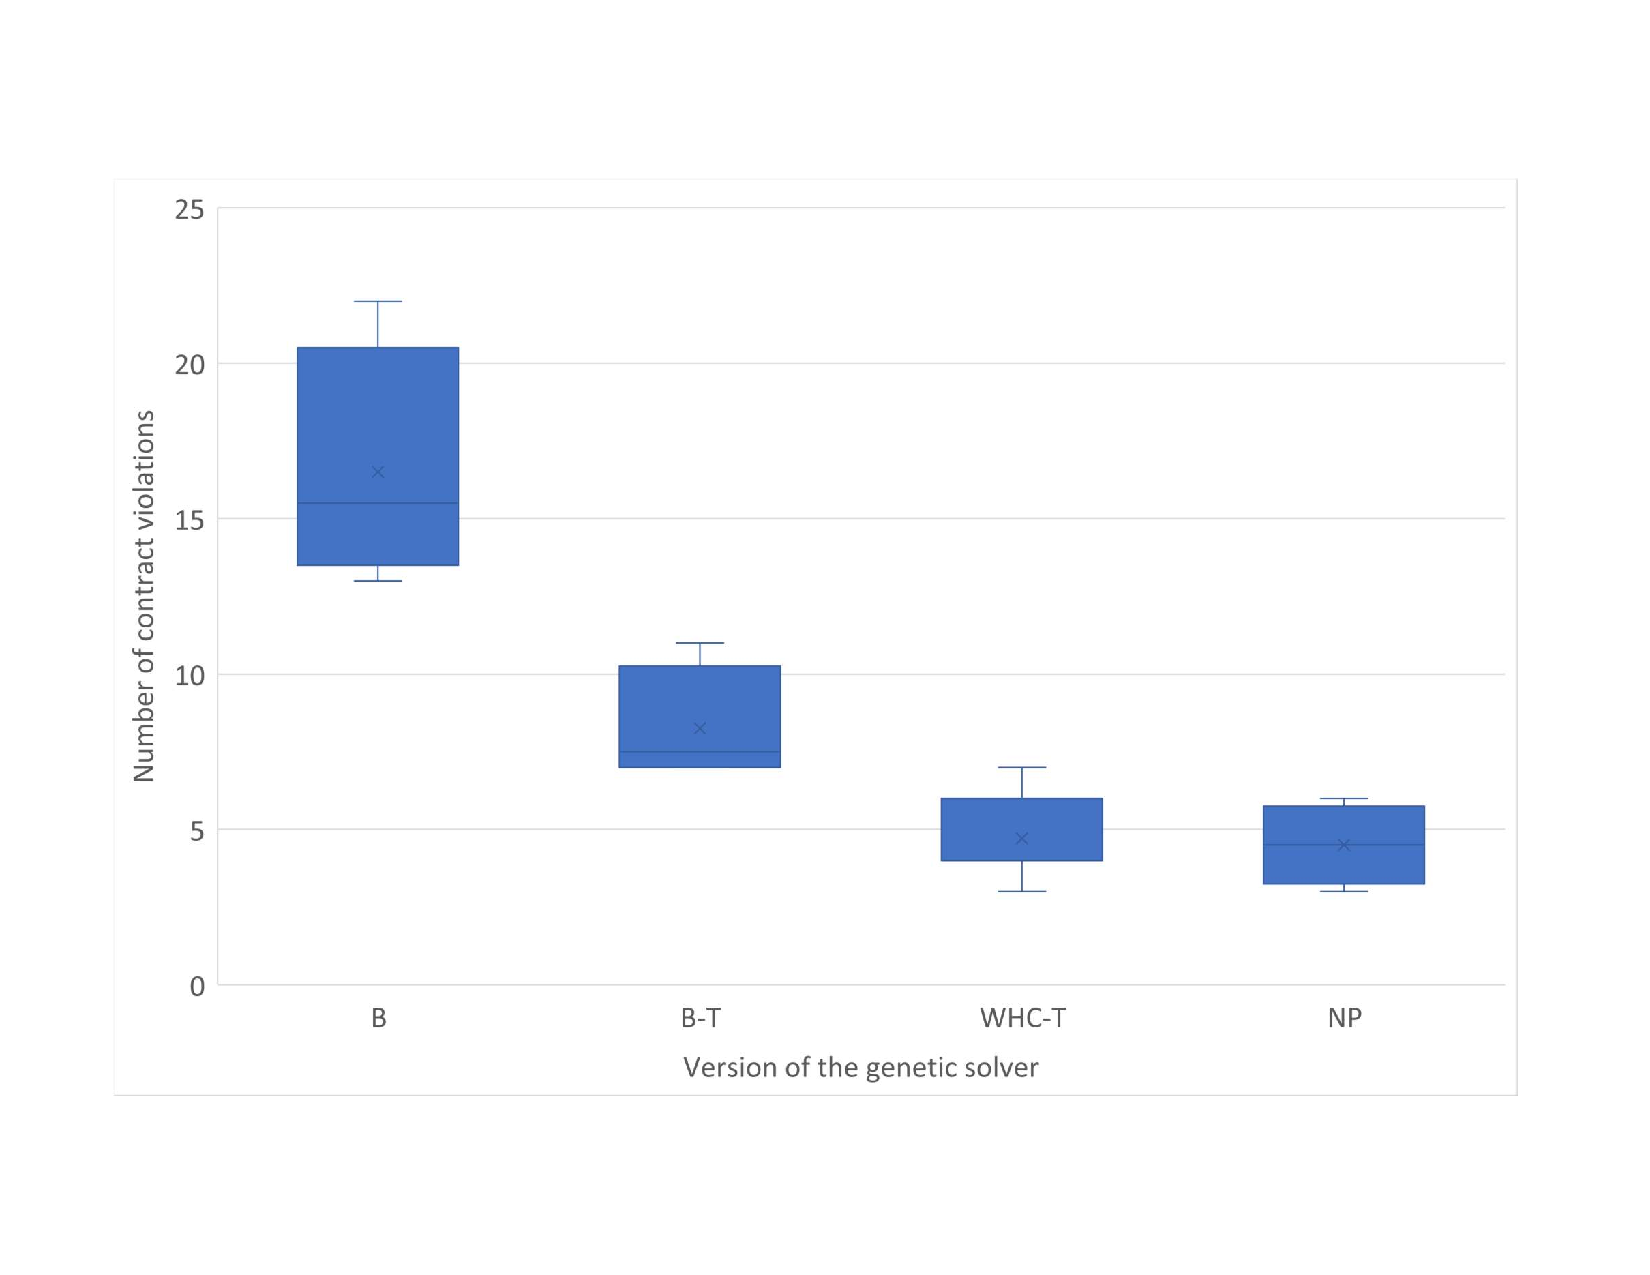
\includegraphics[width=\textwidth]{images/BoxPlotSolverNewParameters.pdf}
	\caption[Box-plot with a number of contract violations for the genetic solver with added probabilities without tuning in comparison with previous versions]{Box-plot with a number of contract violations for the genetic solver with added probabilities without tuning in comparison with previous versions}
	\label{fig:boxplotsolverNewParameters}
\end{figure}

After adding new parameters, we started BRISE to optimize all parameters. The optimized set of parameters is presented in Table~\ref{tab:Parameters_NP-T}. We marked the \textbf{NP} version with optimized set of parameters as \textbf{NP-T}(New Probabilities-Tuned)~\footnote{commit: \href{https://git-st.inf.tu-dresden.de/mquat/mquat2/commit/e103f52b3333900d61c6218a1f2ca811bca10289}{e103f52b3333900d61c6218a1f2ca811bca10289}}. As it was shown, parameter tuning with described parameters returns \textit{NSGA2} as a selector. Moreover, BRISE decide that optimized values of parameters located in the middle of the values range.

\begin{figure}
	\centering
	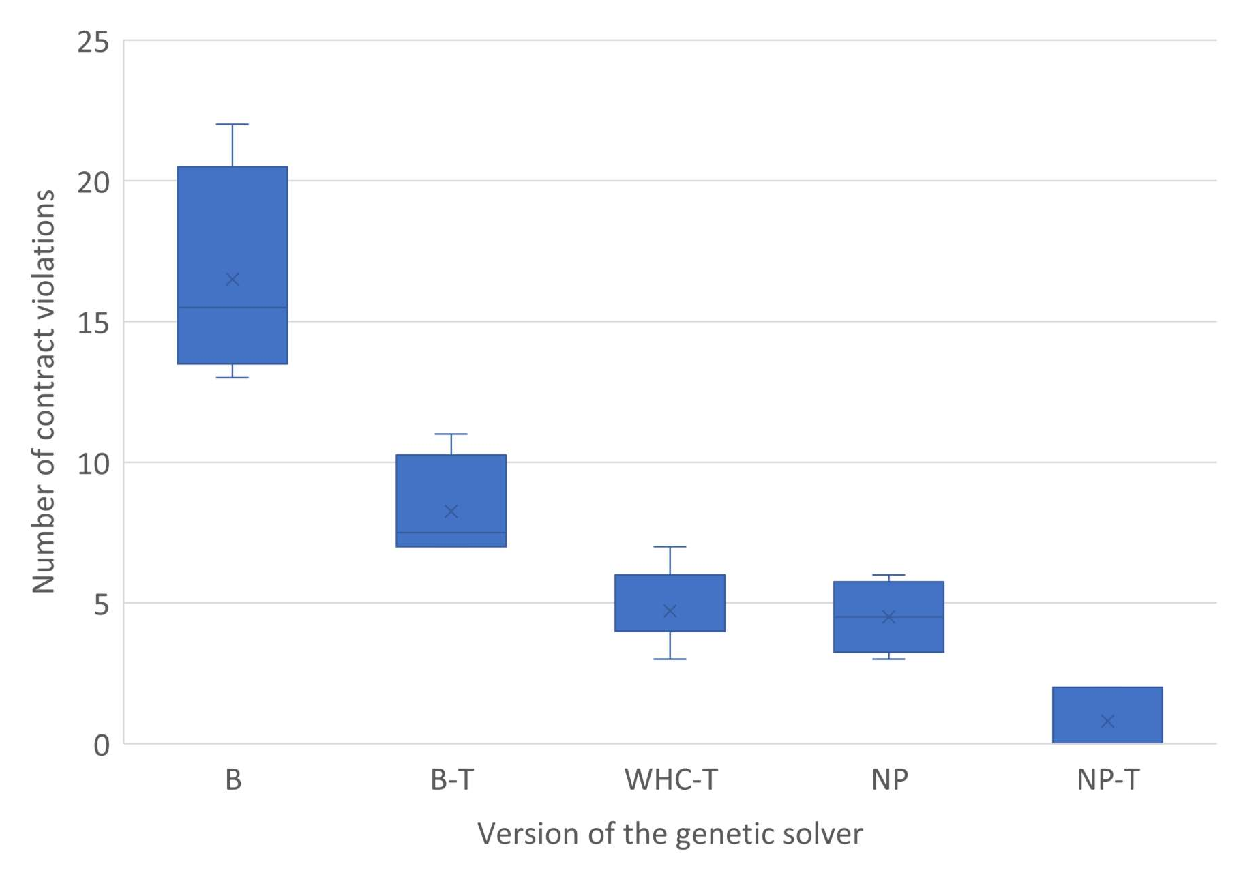
\includegraphics[width=\textwidth]{images/BoxPlotSolverNewParametersTuning.pdf}
	\caption[Box-plot with a number of contract violations for the genetic solver with added probabilities and tuned parameters in comparison with previous versions]{Box-plot with a number of contract violations for the genetic solver with added probabilities and tuned parameters in comparison with previous versions}
	\label{fig:boxplotsolverNewParametersTuning}
\end{figure}

Box-plots in Figure~\ref{fig:boxplotsolverNewParametersTuning} show the comparisons of the NP-T version of the genetic solver to earlier discussed versions~(\textbf{B}, \textbf{B-T}, \textbf{WHC-T}, \textbf{NT}). As shown, the combined approach of parameter engineering and parameter tuning gives a zero number of contract violations. It means that the \textbf{NP-T} version has a \textbf{valid} solution for the MQuAT problem described at the beginning of this chapter. Even the worth-case of the \textbf{NP-T} version with 2 contract violations is better than all versions presented in previous sections. \\ 

This section showed that the parameters thought out in the algorithm are as important as the values of these parameters. If the algorithm is not designed correctly, the tuning parameter may improve the results, but this may not be enough. But not all solutions of the \textbf{NP-T} version are valid. The reason for this is that all versions of the genetic solver that were previously discussed trap into the local optimum.  It could not get out because, at a certain moment, the majority of the individuals in the population becomes the same, and any newly created individual in most cases has worse value of the objective function. But we try to solve it.

\section{Simple parameter control}

The reason why all individuals become the same is the creation of the offspring. To create a new individual, the selector takes the best individuals. Crossover, takes two individuals from the selector, and performs a gene exchange, creating two new individuals. If these individuals give a worse solution, then the selector in the new iteration will drop them, but if they are better, it will take them to create new individuals. At a certain point, there will be a situation that the crossover occurs between two identical genotypes, which creates two identical to parents individuals. There is a case \texttt{1~-~mutationRate} that mutation will not happen, and two identical as parents individuals will be added to the population. It increases the number of identical elements and leads to the collapse of the genetic diversity of the population.

The idea of solving this issue is in internally changeable crossover rate. It changes the chance of the crossover depending on the number of identical individuals in a population. 
The principle of operation is as follows. After each iteration, the ratio of unique genotypes in the population is calculated. If the resulting number is smaller than the value of \texttt{PartOfUniqueIndividualsToStopCrossover}~(R19)~[0.0-1.0]~[Float] parameter, then the probability of a crossover will be set to 0.0, and vice versa, the crossover rate returns its value if the ratio of unique genotypes in the population is bigger than the value of \texttt{PartOfUniqueIndividualsToReturnCrossover}~(R20)~[0.0-1.0]~[Float] parameter.

The value for \texttt{PartOfUniqueIndividualsToStopCrossover} is 0.25 and\linebreak for \texttt{PartOfUniqueIndividualsToReturnCrossover} is 0.75.

The version of the genetic solver with internally changeable crossover rate marked as \textbf{ICCR}(Internally Changeable Crossover Rate)~\footnote{commit: \href{https://git-st.inf.tu-dresden.de/mquat/mquat2/commit/c89422c6e46a5f4e8bc09205df7713ad8fe6907c}{c89422c6e46a5f4e8bc09205df7713ad8fe6907c}} and tuned version~\footnote{commit: \href{https://git-st.inf.tu-dresden.de/mquat/mquat2/commit/128a6f2f844edd70d0e8ee616f09ac897cb86f4e}{128a6f2f844edd70d0e8ee616f09ac897cb86f4e}} was marked as \textbf{ICCR-T}(Internally Changeable Crossover Rate-Tuned).

The parameter sets used for both versions presented in Table~\ref{tab:Parameters_ICCR-T}. If we compare optimized values of parameters from previous section, we can see that \textit{NSGA2} selector changed to \textit{SPEA2}. All other values are the same.

\begin{table}
	\centering
	\caption{Parameters of ICCR and ICCR-T versions of the genetic solver}\label{tab:Parameters_ICCR-T}
	\resizebox{\textwidth}{!}{
		\begin{tabular}{c c c c c c c c c c c c c c c c c c c}
			\hline
			\rotatebox{0}{Genetic solver} & \rotatebox{0}{\texttt{R1}} & \rotatebox{0}{\texttt{R3}} & \rotatebox{0}{\texttt{R4}} & \rotatebox{0}{\texttt{R5}} & \rotatebox{0}{\texttt{R6}} & \rotatebox{0}{\texttt{R7}} & \rotatebox{0}{\texttt{R8}}  &  \rotatebox{0}{\texttt{R10}} & \rotatebox{0}{\texttt{R11}} & \rotatebox{0}{\texttt{R12}} & \rotatebox{0}{\texttt{R13}} &
			\rotatebox{0}{\texttt{R14}} &
			\rotatebox{0}{\texttt{R15}} &
			\rotatebox{0}{\texttt{R16}} &
			\rotatebox{0}{\texttt{R17}} &
			\rotatebox{0}{\texttt{R18}} &
			\rotatebox{0}{\texttt{R19}} &
			\rotatebox{0}{\texttt{R20}} \\
			\hline            
			ICCR & NSGA2 & 500 & 0.1 & 0.95 & 0.1 & 0.45 & 0.5 & 0.5 & 0.5 & 50 & 100 & 0.5 & 0.5 & 0.0 & 0.5 & 0.5 & 0.25 & 0.75 \\
			ICCR-T & SPEA2 & 2550 & 0.5 & 0.5 & 0.5 & 0.5 & 0.5 & 0.5 & 0.5 & 500 & 500 & 0.5 & 0.5 & 0.5 & 0.5 & 0.5 \\
			\hline
		\end{tabular}
	}
\end{table}


\begin{figure}
	\centering
	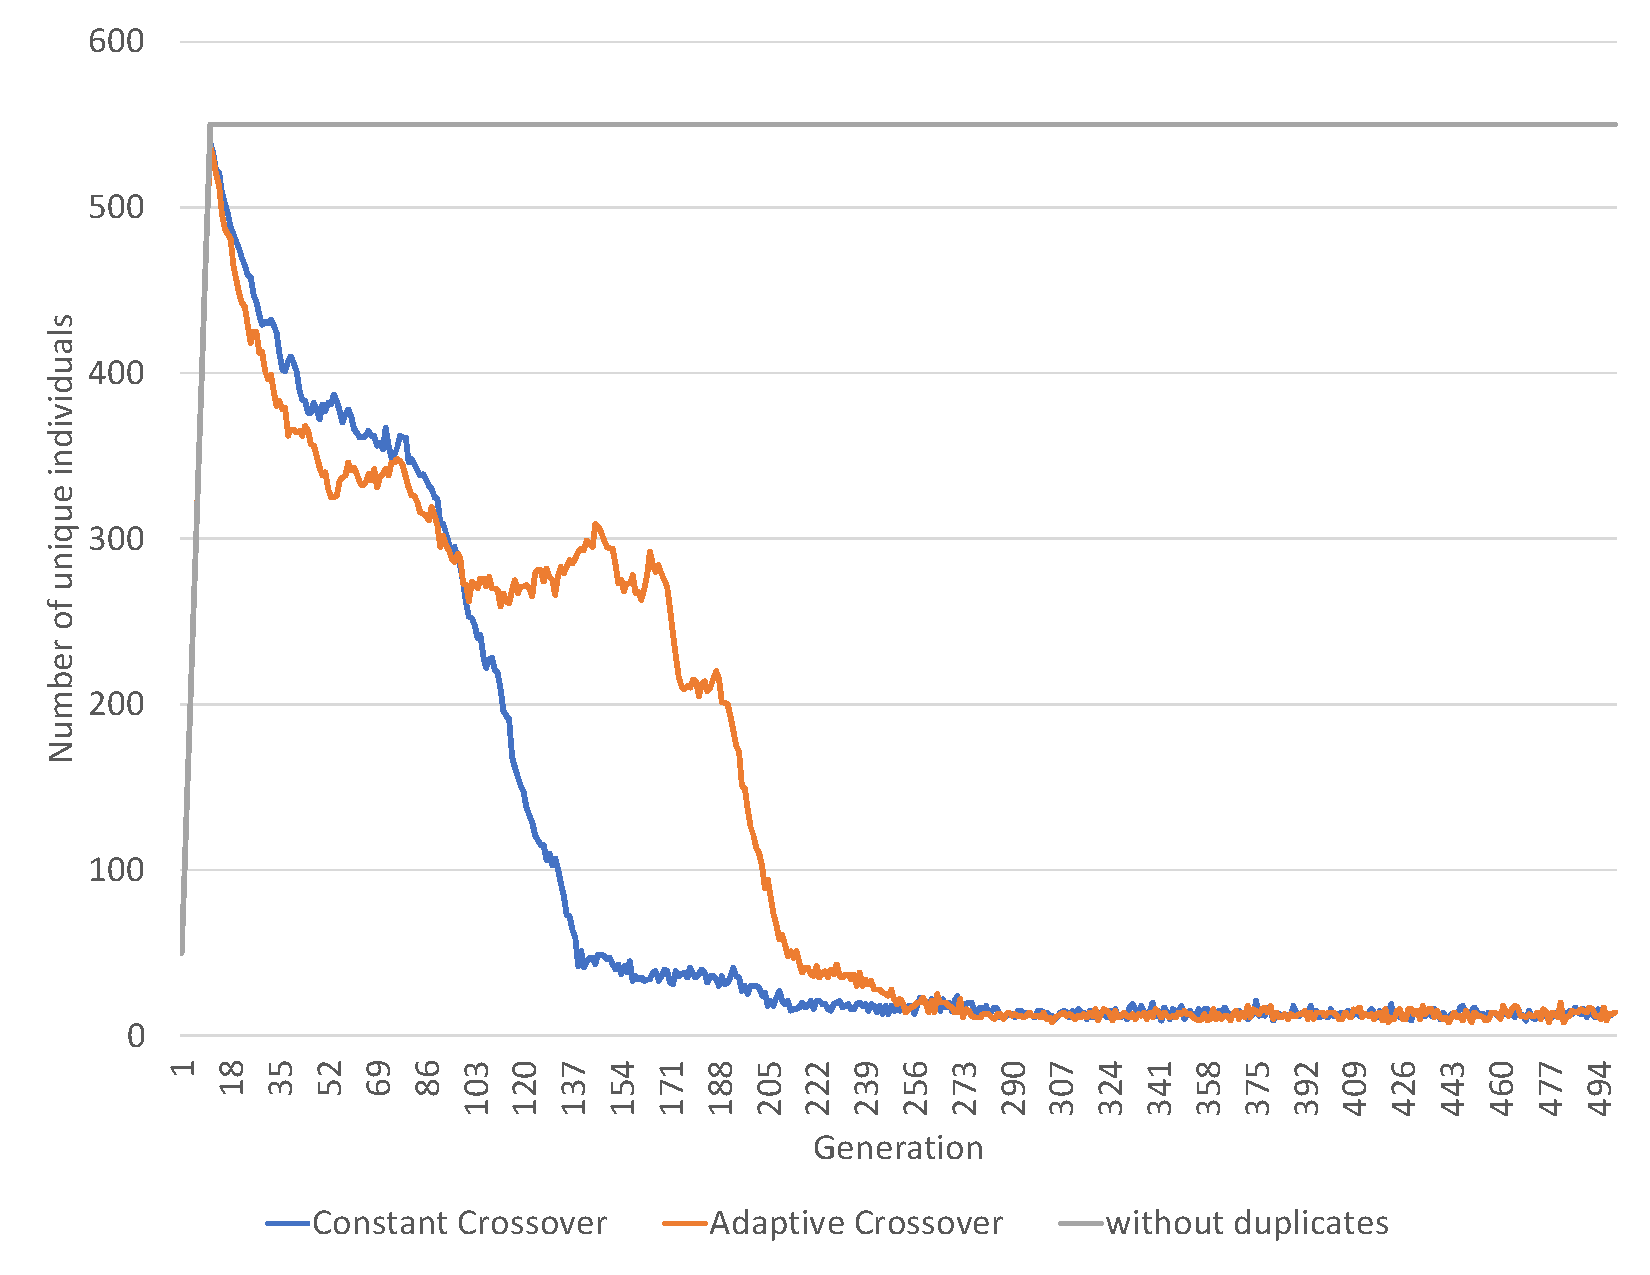
\includegraphics[width=\textwidth]{images/UniqIndividualsPerGeneration3.pdf}
	\caption[]{}
	\label{fig:UniqIndividualsPerGeneration3}
\end{figure} 


The internally changeable crossover rate slightly delay the collapse of the diversity of individuals in the population. Figure~\ref{fig:UniqIndividualsPerGeneration3} shows the deterioration in population diversity for a constant crossover rate and an internally changeable crossover rate.


The comparison of the results of \textbf{ICCR} and \textbf{ICCR-T} versions with all earlier discussed versions is presented as box-plots showed in Figure~\ref{fig:boxplotsolverAdaptiveCrossoverTuning}. The \textbf{ICCR} version gives better results than all untuned versions of the genetic solver. However, the range between max and min number of contract violations in the \textbf{ICCR} version is bigger than in the \textbf{NP} version.
The \textbf{ICCR} also better than tuned versions such as \textbf{B-T} and \textbf{WHC-T}, but worse than the \textbf{NP-T} version. The \textbf{ICCR-T} version as an \textbf{NP-T} version gives a valid solution, but in more like an exception case. The box-plot of the \textbf{ICCR-T} version also shows that parameter tuning for internally changeable parameters works not so efficient as for static parameters like in \textbf{NP} version, at least for the discussed problem. 

\begin{figure}
	\centering
	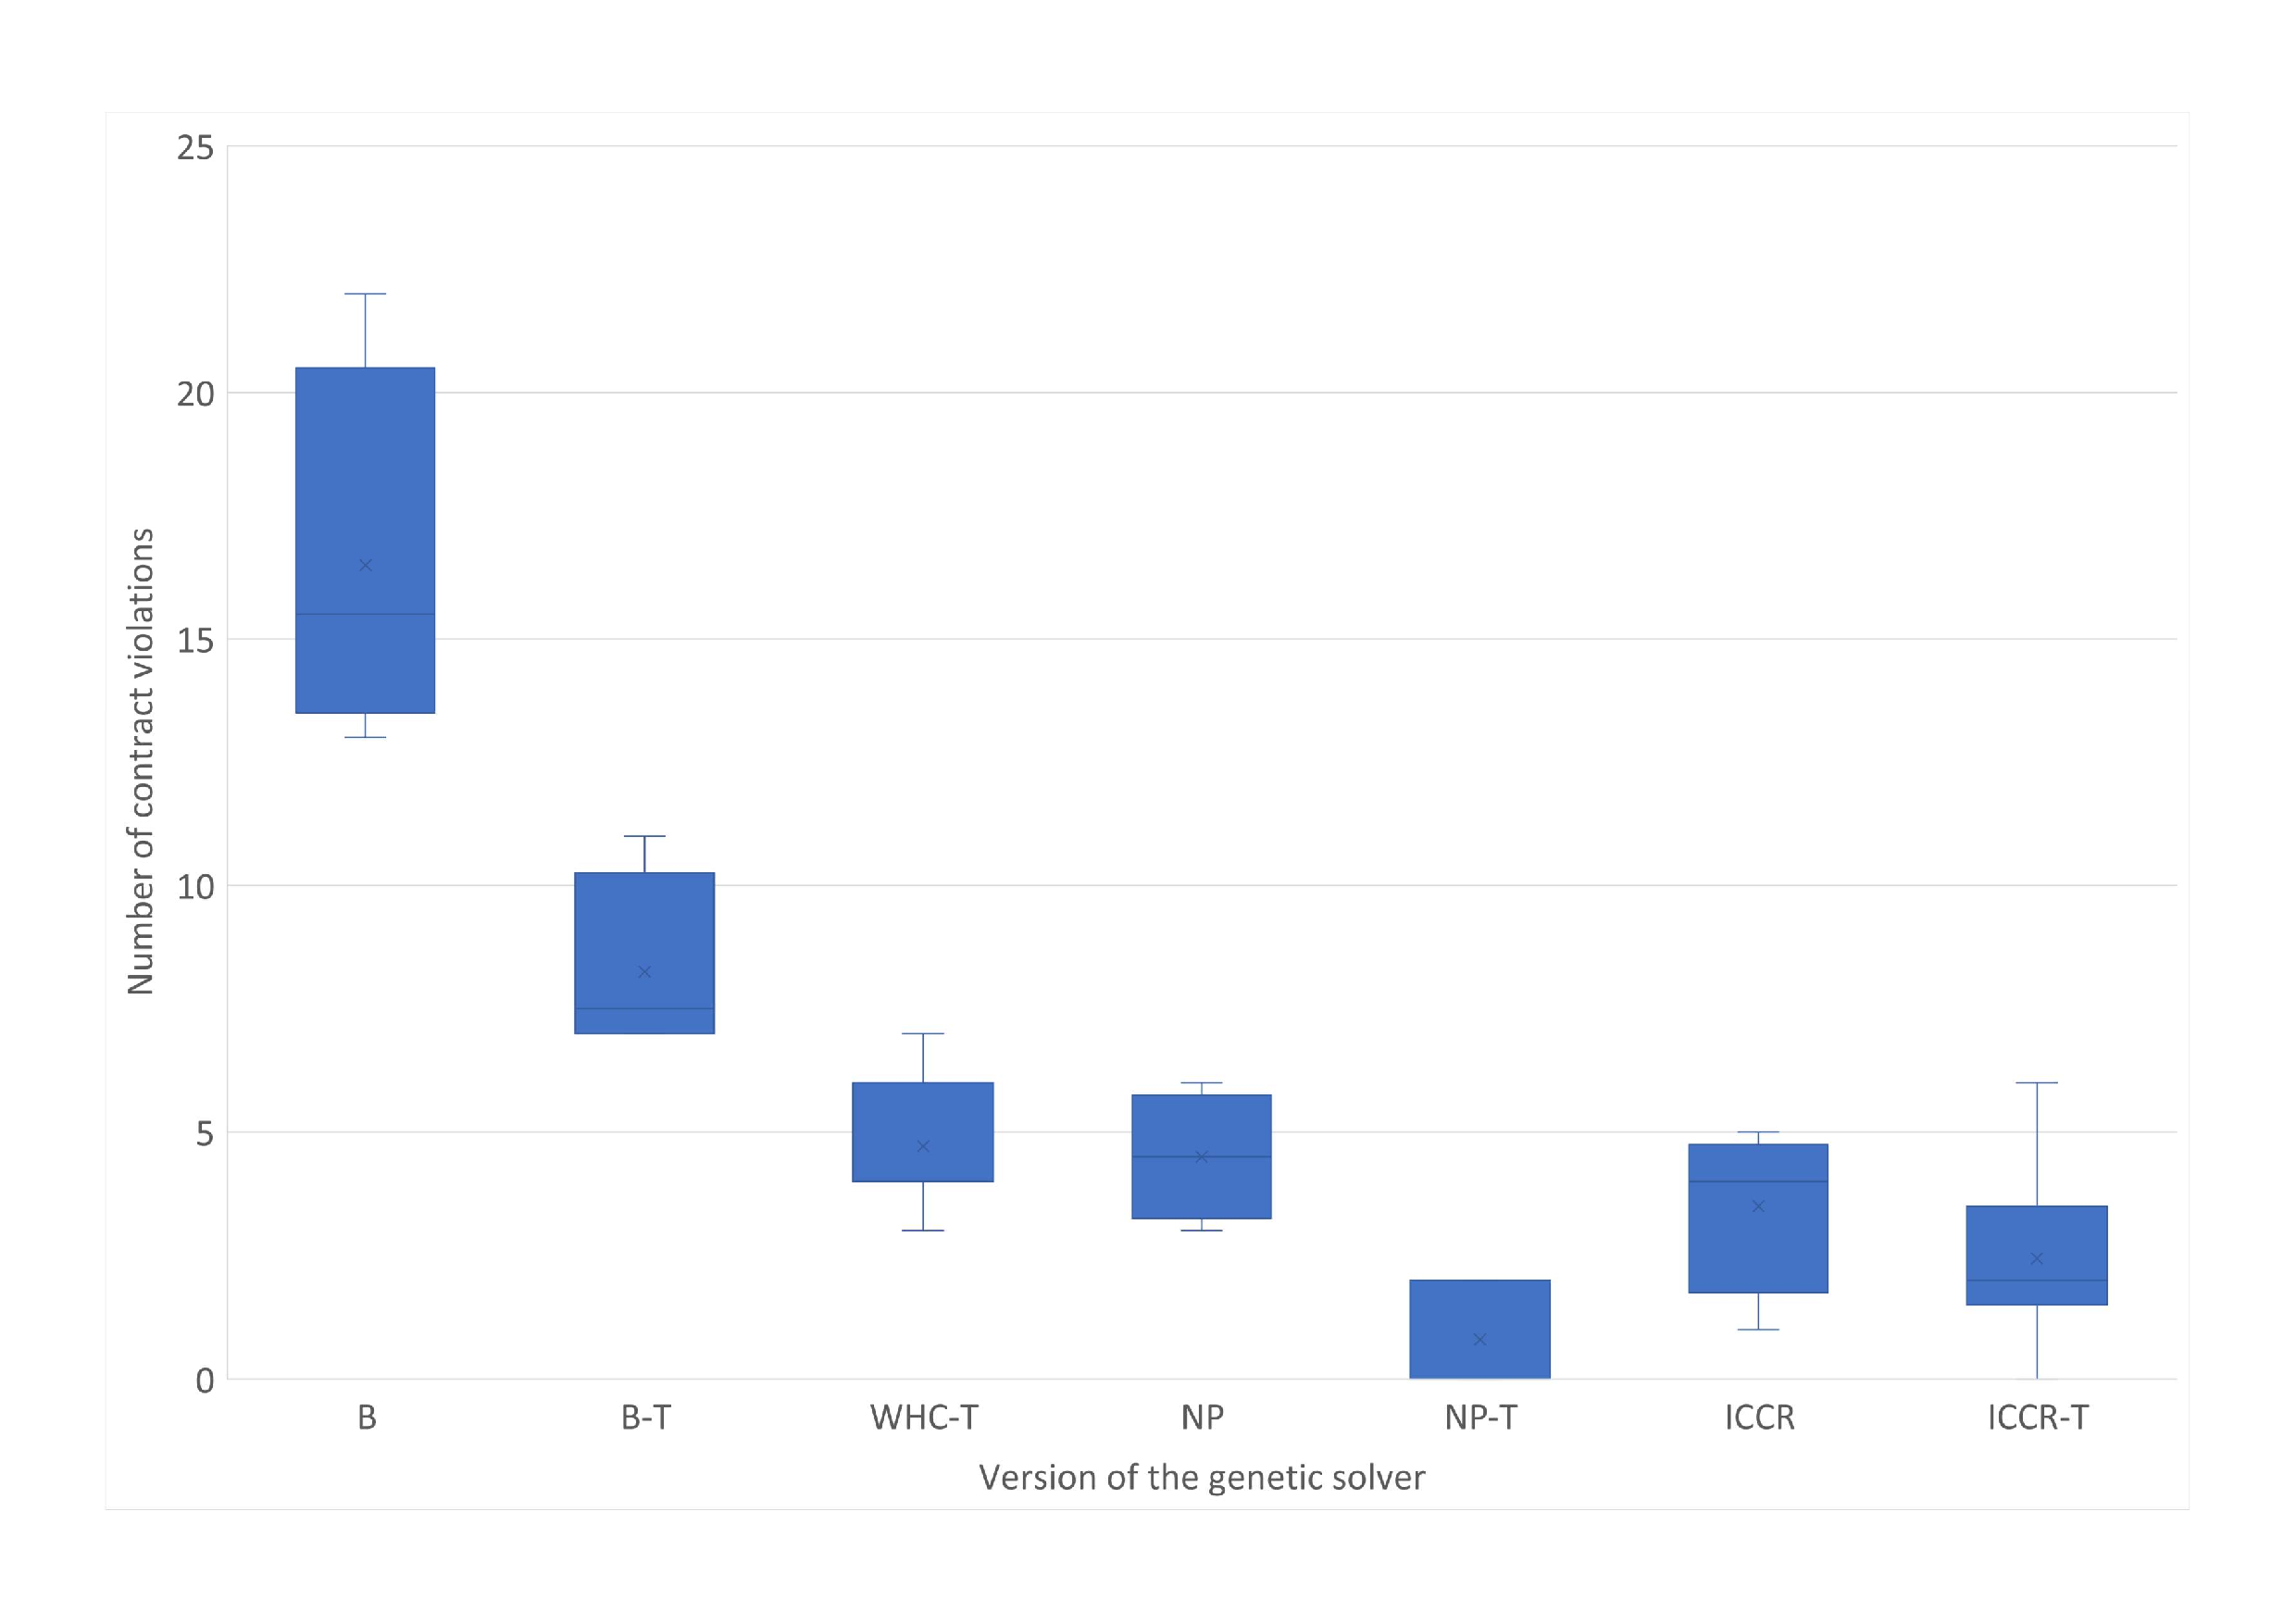
\includegraphics[width=\textwidth]{images/BoxPlotSolverAdaptiveCrossoverTuning.pdf}
	\caption[Box-plot with a number of contract violations for the genetic solver with internally changeable crossover rate in comparison with previously discussed versions]{Box-plot with a number of contract violations for the genetic solver with internally changeable crossover rate in comparison with previously discussed versions}
	\label{fig:boxplotsolverAdaptiveCrossoverTuning}
\end{figure}


This section shows that parameter control could improve the results and postpone stuck in a local optimum. However, parameter tuning for static parameters does not work so well on parameters that change their values during the run-time.                     

\section{Unique genotypes in a population}
\label{sec:WD}

Since the changeable crossover rate from the previous section only delays the collapse of the diversity of individuals in the population, we try a more radical solution. We block the possibility of adding to the population a new individual if the population already contains the same individual. It means that at any moment, the population will consist of unique individuals. In this version of the genetic solver, the use of the changeable crossover rate does not make any sense, so it was disabled, and a constant value was used.

Untuned version of the genetic solver with blocked duplicates in the population marked as  \textbf{WD}~\footnote{commit: \href{https://git-st.inf.tu-dresden.de/mquat/mquat2/commit/1d79c50d7932c9216c653bf6d0354d990f6aecbc}{1d79c50d7932c9216c653bf6d0354d990f6aecbc}}~(Without Duplicates) and tuned version~\footnote{commit: \href{https://git-st.inf.tu-dresden.de/mquat/mquat2/commit/24504c77024ac383c77849c5121471e0f06ce913}{24504c77024ac383c77849c5121471e0f06ce913}} marked as \textbf{WD-T}~(Without Duplicates-Tuned).

The number of unique individuals in the population for the WD version presented in Figure~\ref{fig:UniqIndividualsPerGeneration3}. In each generation, after the initial population has been created, the number of unique elements in the population is not changing.



Parameters for both versions presented in Table~\ref{tab:Parameters_WD-T}.


\begin{table}
	\centering
	\caption{Parameters of WD and WD-T versions of the genetic solver}\label{tab:Parameters_WD-T}
	\resizebox{\textwidth}{!}{
		\begin{tabular}{c c c c c c c c c c c c c c c c c}
			\hline
			\rotatebox{0}{Genetic solver} & \rotatebox{0}{\texttt{R1}} & \rotatebox{0}{\texttt{R3}} & \rotatebox{0}{\texttt{R4}} & \rotatebox{0}{\texttt{R5}} & \rotatebox{0}{\texttt{R6}} & \rotatebox{0}{\texttt{R7}} & \rotatebox{0}{\texttt{R8}}  &  \rotatebox{0}{\texttt{R10}} & \rotatebox{0}{\texttt{R11}} & \rotatebox{0}{\texttt{R12}} & \rotatebox{0}{\texttt{R13}} &
			\rotatebox{0}{\texttt{R14}} &
			\rotatebox{0}{\texttt{R15}} &
			\rotatebox{0}{\texttt{R16}} &
			\rotatebox{0}{\texttt{R17}} &
			\rotatebox{0}{\texttt{R18}} \\
			\hline            
			WD & NSGA2 & 500 & 0.1 & 0.95 & 0.1 & 0.45 & 0.5 & 0.5 & 0.5 & 50 & 100 & 0.5 & 0.5 & 0.0 & 0.5 & 0.5 \\
			WD-T & SPEA2 & 1057 & 0.49 & 0.66 & 0.82 & 0.04 & 0.95 & 0.09 & 0.04 & 929 & 383 & 0.68 & 0.85 & 0.51 & 0.41 & 0.65 \\
			\hline
		\end{tabular}
	}
\end{table}

\begin{figure}
	\centering
	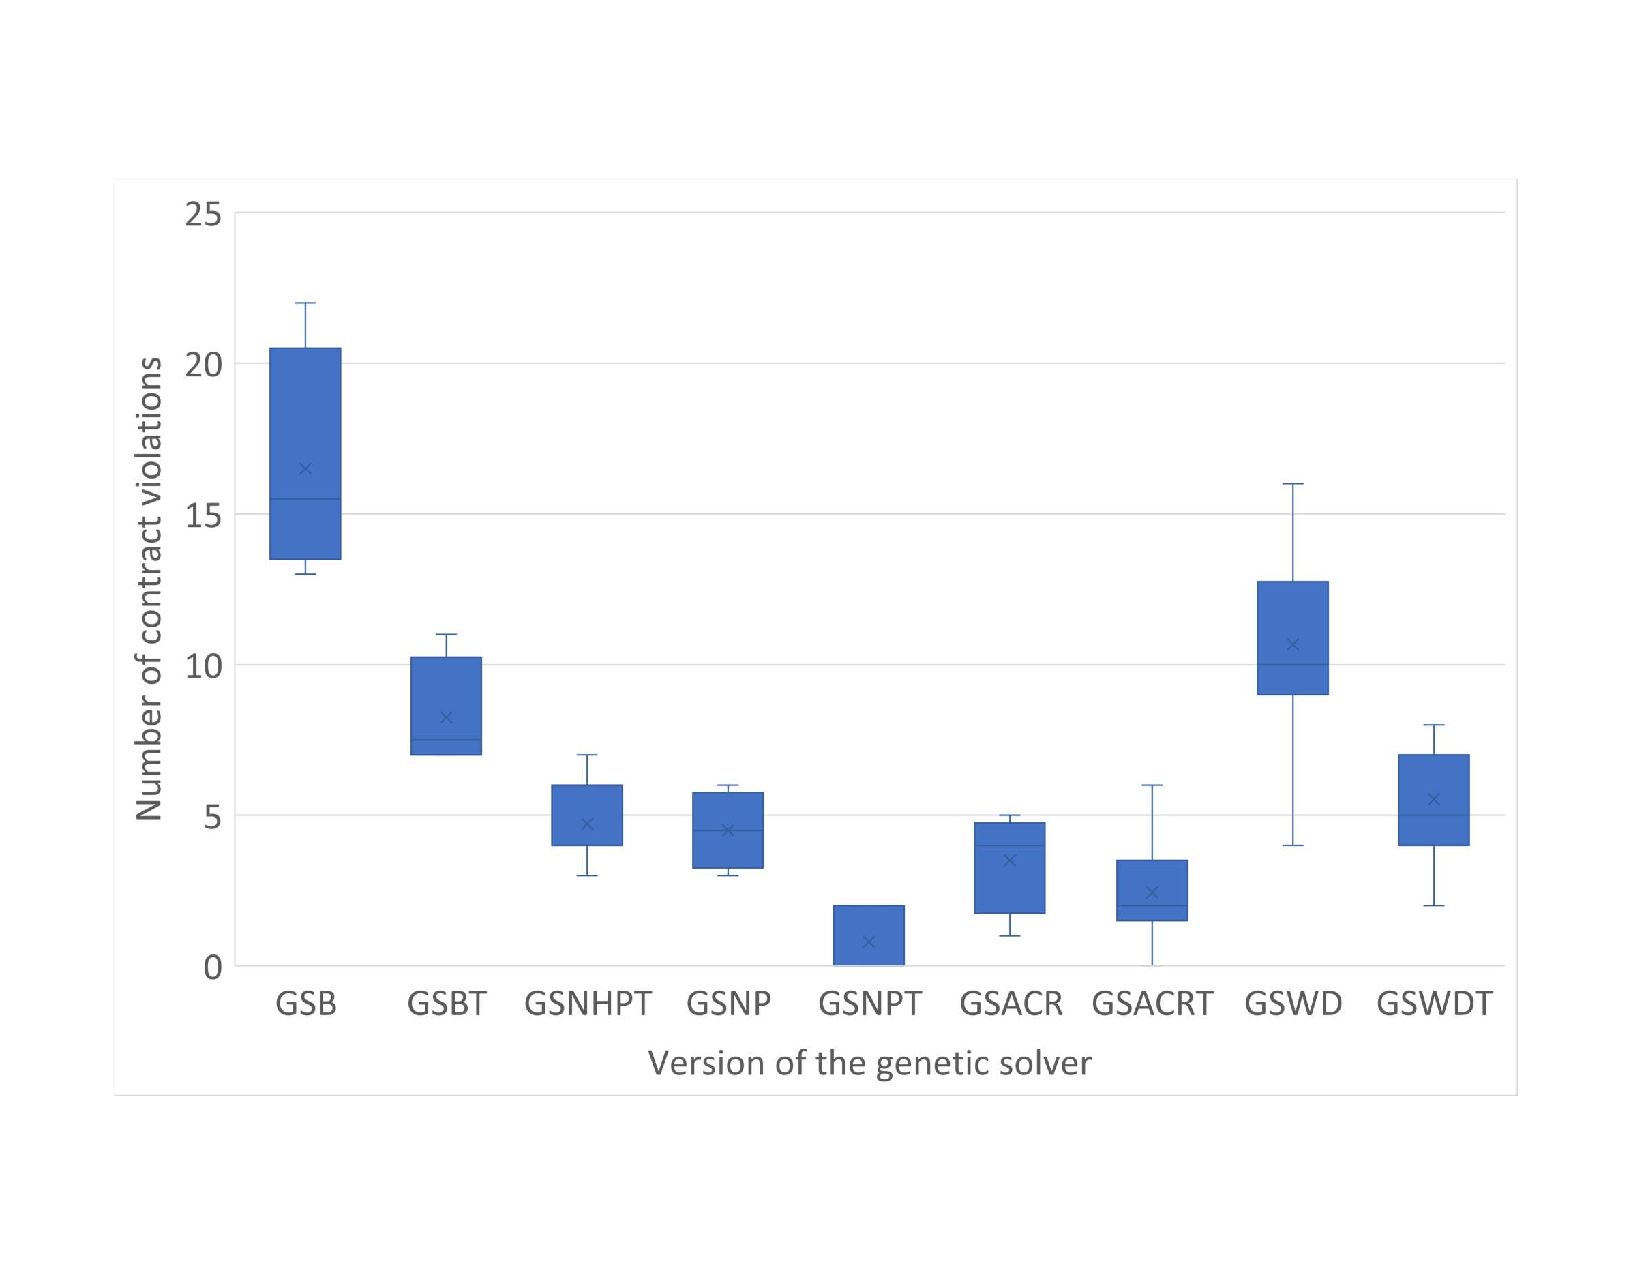
\includegraphics[width=\textwidth]{images/BoxPlotSolverNoDuplicates.pdf}
	\caption[Boxplot with a number of contract violations for the genetic solver without duplicates in the population in comparison with previous versions]{Boxplot with a number of contract violations for the genetic solver without duplicates in the population in comparison with previous versions}
	\label{fig:boxplotsolverNoDuplicates}
\end{figure} 

Figure~\ref{fig:boxplotsolverNoDuplicates} shows the results of this approach with and without parameter tuning. Obtained results show that the WD version of the genetic solver gives better results only in comparison to the B version and not always. The WD-T version gives better results with less range between min and max number of contract violations than WD. But it much worse than NP-T.

There are two main reasons why the results of this approach are much worse than previous versions. The first one is a calculation speed. It is slower than in previous versions. As a result, the number of created generations is lower. For the NP version, this number is 15177. For the WD version, this number is 2605, more than five times less according to our tests.

The second reason is a few "good" individuals selected to create offspring. This number is low because the selector could select the best individual from the population only once per selection. As a result, selected the best individual could give a few new individuals. Theoretically, the small value of the \texttt{mu} parameter could help. Nevertheless, BRISE gives the value of the \texttt{mu} parameter even higher than the default value. 

The conclusion of this idea is quite pessimistic because other approaches work better on this problem, but it may work better than others with different problems or on long term optimization.


\begin{table}
	\centering
	\caption{Parameters of NP and NP-T versions of the genetic solver}\label{tab:Parameters_all_versions}
	\resizebox{\textwidth}{!}{
		\begin{tabular}{c c c c c c c c c c c c c c c c c c c c}
			\hline
			\rotatebox{0}{Genetic solver} & \rotatebox{0}{\texttt{R1}} & \rotatebox{0}{\texttt{R3}} & \rotatebox{0}{\texttt{R4}} & \rotatebox{0}{\texttt{R5}} & \rotatebox{0}{\texttt{R6}} & \rotatebox{0}{\texttt{R7}} & \rotatebox{0}{\texttt{R8}}  & \rotatebox{0}{\texttt{R9}}  & \rotatebox{0}{\texttt{R10}} & \rotatebox{0}{\texttt{R11}} & \rotatebox{0}{\texttt{R12}} & \rotatebox{0}{\texttt{R13}} &
			\rotatebox{0}{\texttt{R14}} &
			\rotatebox{0}{\texttt{R15}} &
			\rotatebox{0}{\texttt{R16}} &
			\rotatebox{0}{\texttt{R17}} &
			\rotatebox{0}{\texttt{R18}} &
			\rotatebox{0}{\texttt{R19}} &
			\rotatebox{0}{\texttt{R20}} \\
			\hline            
			B & NSGA2 & 500 & \cellcolor{Gray} 0.1 & \cellcolor{Gray} 0.95 & \cellcolor{Gray} 0.1 & \cellcolor{Gray} 0.45 & \cellcolor{Gray} 0.5 & \cellcolor{Gray} 0.8 & \cellcolor{Gray} 0.5 & \cellcolor{Gray} 0.5 & \cellcolor{Gray} 50 & \cellcolor{Gray} 100 \\
			
			B-T & NSGA2 & 1533 & \cellcolor{Gray} 0.1 & \cellcolor{Gray} 0.95 & \cellcolor{Gray} 0.1 & \cellcolor{Gray} 0.45 & \cellcolor{Gray} 0.5 & \cellcolor{Gray} 0.8 & \cellcolor{Gray} 0.5 & \cellcolor{Gray} 0.5 & \cellcolor{Gray} 50 & \cellcolor{Gray} 100 \\    
			
			WHC-T & SPEA2 & 2014 & 0.98 & 0.95 & 0.58 & 0.02 & 0.64 & 0.3 & 0.95 & 0.17 & 79 & 266 \\
			
			NP & NSGA2 & 500 & 0.1 & 0.95 & 0.1 & 0.45 & 0.5 & & 0.5 & 0.5 & 50 & 100 & 0.5 & 0.5 & 0.0 & 0.5 & 0.5 \\
			
			NP-T & NSGA2 & 2550 & 0.5 & 0.5 & 0.5 & 0.5 & 0.5 & & 0.5 & 0.5 & 500 & 500 & 0.5 & 0.5 & 0.5 & 0.5 & 0.5 \\
			
			ICCR & NSGA2 & 500 & 0.1 & 0.95 & 0.1 & 0.45 & 0.5 & & 0.5 & 0.5 & 50 & 100 & 0.5 & 0.5 & 0.0 & 0.5 & 0.5 & 0.25 & 0.75 \\
			
			ICCR-T & SPEA2 & 2550 & 0.5 & 0.5 & 0.5 & 0.5 & 0.5 & & 0.5 & 0.5 & 500 & 500 & 0.5 & 0.5 & 0.5 & 0.5 & 0.5 & 0.5 & 0.5 \\
			
			WD & NSGA2 & 500 & 0.1 & 0.95 & 0.1 & 0.45 & 0.5 & & 0.5 & 0.5 & 50 & 100 & 0.5 & 0.5 & 0.0 & 0.5 & 0.5 \\
			
			WD-T & SPEA2 & 1057 & 0.49 & 0.66 & 0.82 & 0.04 & 0.95 & & 0.09 & 0.04 & 929 & 383 & 0.68 & 0.85 & 0.51 & 0.41 & 0.65 \\
			\hline
		\end{tabular}
	}
\end{table}

\begin{figure}
	\centering
	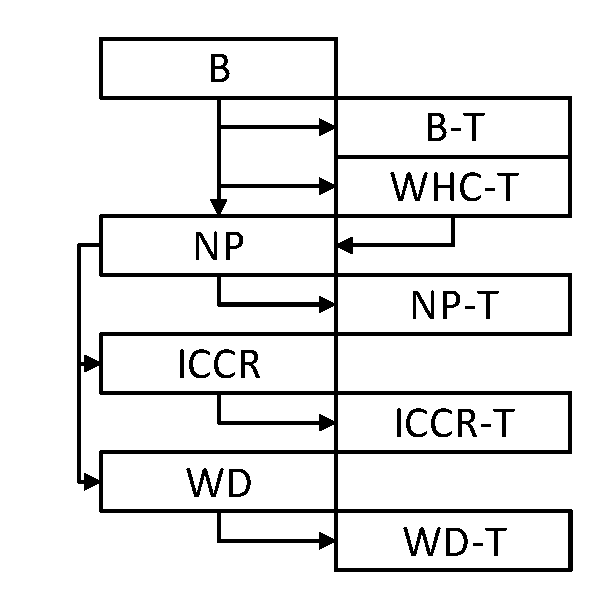
\includegraphics[width=0.5\textwidth]{images/GSVersions.pdf}
	\caption[Version history of Genetic Solver]{Version history of Genetic Solver}
	\label{fig:GSVersions}
\end{figure} 


